%!TEX encoding = UTF8
%!TEX root =notes.tex

\chapter{Droite réelle et géométrie plane}

\section{Droite réelle}
	

On considère la droite graduée suivante.

\begin{center}
	
	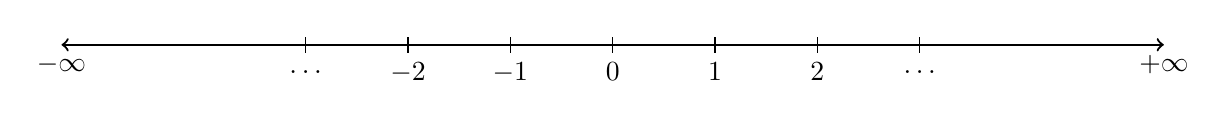
\begin{tikzpicture}
		
		% real line
		\draw[<->, thick] (-7,0) node[below] {$-\infty$} -- (7,0) node[below] {$+\infty$};
		
		\foreach \x in {-2,...,2}
			\draw[-] (1.3*\x,-.1) node[below] {$\x$} -- (1.3*\x,.1) node{};
		
		\foreach \x in {-3, 3}
			\draw[-] (1.3*\x,-.1) node[below=3pt] {$\dots$} -- (1.3*\x,.1) node{};
		
	
	\end{tikzpicture}
\end{center}

On peut construire à la règle et au compas le nombre $\sqrt{2}$ sur la droite grâce au théorème de Pythagore.

\exe{}{
	Construire, en utilisant uniquement la règle et le compas, tous les nombres rationnels, c'est-à-dire toutes les fractions $\dfrac{p}q$ où $p, q \in \Z$ et $q \neq 0$.
	
	\emph{Indication : les couples $(1, p/q)$ et $(q, p)$ sont proportionnels.}
}

L'ensemble des points de la droite est donc strictement plus grand que celui des rationnels, car $\sqrt{2}$ n'est pas rationnel d'après le théorème \ref{thm:1}.

\begin{center}
	
	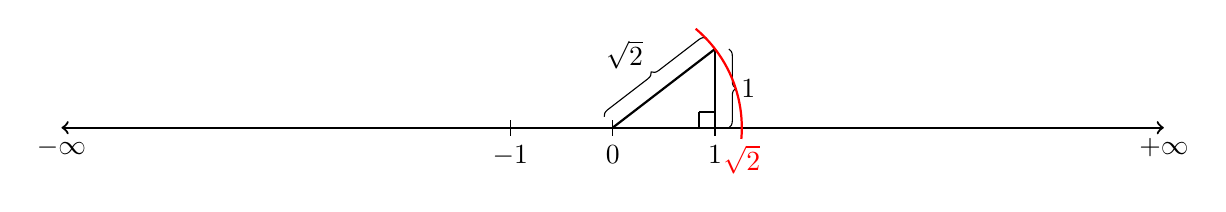
\begin{tikzpicture}
		
		% real line
		\draw[<->, thick] (-7,0) node[below] {$-\infty$} -- (7,0) node[below] {$+\infty$};
		\foreach \x in {-1, 0, 1}
			\draw[-] (1.3*\x,-.1) node[below] {$\x$} -- (1.3*\x,.1);
		
		% right angled triangle
		\draw[-, thick] (1.3,0) -- (1.3,1);
		\draw[-, thick] (0,0)-- (1.3,1);
		
		\draw[-, thick] (1.1,0)-- (1.1,.2);
		\draw[-, thick] (1.1,.2)-- (1.3,.2);
		
		% lengths
		\draw[decoration={brace,raise=5pt},decorate]
  			(0,0) -- node[above=12pt, left=4pt] {$\sqrt{2}$} (1.3,1);
		\draw[decoration={brace,mirror,raise=5pt},decorate]
  			(1.3,0) -- node[right=6pt] {$1$} (1.3,1);
  			
  			
		% circle arc
		 \draw [red,thick,domain=-5:50] plot ({sqrt(2.69)*cos(\x)}, {sqrt(2.69)*sin(\x)});
		 
		 % sqrt{2} mark
		\draw[-, red] (1.640,-.1) node[below, red] {$\sqrt{2}$} -- (1.640,.1);
				
	\end{tikzpicture}
\end{center}

Tous les points de la droite ne peuvent en fait pas être construit à la règle et au compas. Ceci est étroitement lié au théorème de Gauss-Wantzel sur les	polygônes réguliers constructibles.
En particulier, l'heptagone régulier n'est pas constructible à la règle et au compas.
	
Ce théorème est en dehors du champ d'application du cours.

\dfn{Nombres réels $\R$}{
	À chaque point de la droite on associe un nombre, appelé \emph{réel}.
	L'ensemble des nombres réels est noté $\R$.
}

\nt{
	On a la suite d'inclusions suivantes :
		\[ \N \subset \Z \subset \D \subset \Q \subset \Q. \]
}

\subsection{Intervalles}

\dfn{Intervalle borné}{
	Un intervalle borné est un segment de la droite réelle $\R$. C'est donc un ensemble de nombres.
	Il est donné par une \emph{borne inférieure} $a \in \R$ et une \emph{borne supérieure} $b\in\R$ et peut contenir ou non ses bornes.
	
	\begin{enumerate}
		\item Si $a$ et $b$ sont contenues dans l'intervalle, on le note $[a ; b]$.
		\item Si $a$  est contenue dans l'intervalle mais $b$ ne l'est pas, on le note $[a ; b [$.
		\item Si $a$ n'est pas contenue dans l'intervalle mais $b$ l'est, on le note $] a ; b]$.
		\item Si ni $a$ ni $b$ ne sont contenues dans l'intervalle, on le note $] a ; b [$.
	\end{enumerate}
}
\ex{}{
	Les intervalles suivants sont bornés.
	\begin{multicols}{2}
	\begin{enumerate}[label=$\bullet$]
		\item $[-1 ; 1]$
		\item $[-3 ; 1[$
		\item $]-10{,}341 ; \pi]$
		\item $]\sqrt{2} ; 130[$
	\end{enumerate}
	\end{multicols}

}{}

\dfn{Intervalle non borné}{
	Un intervalle n'est pas forcément borné : une ou les deux bornes peuvent être infinies ($\pinfty$ ou $\minfty$). 
	Dans ce cas, l'intervalle n'inclut jamais l'infini car ce n'est pas un nombre.
}

\ex{}{
	Les intervalles suivants ne sont pas bornés.
	\begin{multicols}{2}
	\begin{enumerate}[label=$\bullet$]
		\item $]\minfty; 2]$
		\item $]\minfty ; 3[$
		\item $]0; \pinfty[$
		\item $\R = ]\minfty; \pinfty[$
	\end{enumerate}
	\end{multicols}
}{ex:3.5}

\subsection{Intersection et union}

\dfn{Intersection, union}{
	Pour deux ensembles $I, J$ on définit les ensembles suivants.
		\begin{enumerate}
			\item $I \cap J$ : l'intersection des deux intervalles.
			
			Un élément appartient à $I \cap J$ dès qu'il appartient à $I$ \textbf{et} à $J$.
			\item $I \cup J$ : l'union des deux intervalles.
			
			Un élément appartient à $I \cup J$ dès qu'il appartient à $I$ \textbf{ou} à $J$.
		\end{enumerate}
	
}


\exe{}{
	Exprimer les intersections et unions suivantes sous forme d'intervalle.
	\begin{multicols}{2}
	\begin{enumerate}
		\item $[-1 ; 1] \cap [-3 ; 1]$
		\item $] {-}\infty ; 2] \cap [-3 ; -2]$
		\item $]{-}\infty ; 4 [ \cup [2 ; +\infty[$
		\item $]-2 ; 4 [  \cup [4 ; 8[$
	\end{enumerate}
	\end{multicols}
}

\subsection{Inégalités}

Un intervalle n'a de sens que si la borne inférieure est plus petite que la borne supérieure.
De plus, un élément appartient à l'ensemble dès qu'il est plus petit que la borne supérieure, et plus grand que la borne inférieure.

Il faut donc pouvoir noter simplement les relations \og plus petit que \fg et \og plus grand que \fg.

\dfn{Inégalités}{
	On définit les signes suivants correspondant à des inégalités \emph{strictes} et \emph{larges}.
		\begin{enumerate}
			\item $<$ : strictement inférieur à
			\item $\leq$ : inférieur ou égal à
			\item $>$ : strictement supérieur à
			\item $\geq$ : supérieur ou égal à
		\end{enumerate}
}

\ex{}{
	\begin{multicols}{3}
	\begin{enumerate}
		\item $1 \leq 2$
		\item $-3 \leq -2$
		\item $0 \leq 0$
		\item $1{,}02 < 1{,}1$
		\item $7{,}391 > 7{,}30001$
		\item $-4{,}001 > -4{,}0001$
	\end{enumerate}
	\end{multicols}
}{}

\nt{
	Appartenir à un intervalle est donc équivalent à respecter certaines inégalités.
	En particulier : être inférieur à la borne supérieure, et être supérieur à la borne inférieure.
	
	On a donc l'équivalence suivante.
		\[ x \in [a ; b] \qquad \iff \qquad x \in \R, x \geq a, \text{ et } x \leq b. \]
		
	On peut noter deux inégalités sur la même lignes dès qu'elles vont dans le même sens.
	Par exemple, les deux inégalités ci-dessus peuvent être condensées en une :
		\[ x \in \R, \text{ et } a \leq x \leq b, \]
	ou encore
		\[ x \in \R, \text{ et } b \geq x \geq a. \]
}

\ex{}{
	\begin{enumerate}
		\item Prendre $x \in [-3 ; 4]$ est équivalent à prendre $x \in \R$ vérifiant $-3 \leq x \leq 4$.
		\item Prendre $x \in [-4 ; 3[$ est équivalent à prendre $x \in \R$ vérifiant $-4 \leq x < 3$.
		\item Prendre $x \in ]\minfty ; 0[$ est équivalent à prendre $x \in \R$ vérifiant $x < 0$.
		
		On dit alors que $x$ est strictement négatif.
		\item Prendre $x \in [0; \pinfty [$ est équivalent à prendre $x \in \R$ vérifiant $x \geq 0$.
		
		On dit alors que $x$ est positif ou nul.
		\item Prendre $x \in ]\minfty; \pinfty[$ est équivalent à prendre $x \in \R$.	
		
		Ceci est en fait tautologique car $]\minfty; \pinfty[ = \R$, comme vu dans l'exemple \ref{ex:3.5}.
	\end{enumerate}
}{}


\subsection{Valeur absolue}

La valeur absolue correspond à la notion de \emph{distance} parmis les réels.
Celle-ci intervient notamment lorsqu'on souhaite calculer la longueur d'un intervalle borné afin de mesure sa précision.
Par exemple, l'intervalle $[1 ; 3]$, dans lequel $2$ appartient, est moins précis que l'intervalle $[1{,}99 ; 2{,}01]$ car sa longueur est plus grande.

Les intervalles de confiance seront étudiés plus tard dans le chapitre dédié aux statistiques.

\exe{}{
	Quelle est la distance dans les réels 
		\begin{multicols}{2}
		\begin{enumerate}
			\item $3$ et $2$ ?
			\item $2$ et $4$ ?
			\item $-1$ et $1$ ?
			\item $-4{,}2$ et $-4{,}12$ ?
		\end{enumerate}
		\end{multicols}
}

\dfn{Valeur absolue}{
	La valeur absolue d'un $x \in \R$ général est égale à $x$ si celui-ci est positif, et à son opposé $-x$ sinon.
	La valeur absolue est donc toujours positive et peut être définie comme suit.
	
		\[ |x| = \begin{cases} x \text{ si $x \geq 0$}, \\ -x \text{ sinon.} \end{cases}. \]

	Soient $a, b \in \R$ deux réels quelconques.
	La distance de $a$ à $b$ est égale à
		\[ \text{Distance entre $a$ et $b$} = \begin{cases} a-b \text{ si $a \geq b$} , \\ b-a \text{ sinon.} \end{cases}. \]
	La condition $a \geq b$ peut être réécrite comme $a-b \geq 0$.
	
	En remarquant que $b-a = -(a-b)$, on voit que la distance entre $a$ et $b$ est exactement donnée par la valeur absolue de $a-b$.
		\[ \text{Distance entre $a$ et $b$} = | a- b|. \]
}

\nt{
	On retrouve d'ailleurs $|x| = |x - 0|$, la distance de $x$ à $0$.
}

\exe{}{
		Quels réels $x\in\R$ vérifient les conditions suivantes ? Donner des ensembles ou des intervalles.
		\begin{multicols}{2}
		\begin{enumerate}
			\item $|x| = 1$
			\item $|2x -4| = 5$
			\item $| x | \leq 3{,}14$
			\item $| 7 + 3x | \leq 10$
		\end{enumerate}
		\end{multicols}
}





\section{Géométrie plane}